\documentclass[12pt]{article}
\usepackage[none]{hyphenat}
%\usepackage[T1]{fontenc}
\usepackage{polski}
\usepackage[utf8]{inputenc}
\usepackage{amsmath}
\usepackage{amssymb}
\usepackage{graphicx}
\usepackage{program}
%\usepackage{enumerate}
%\usepackage{verbatim}
\usepackage{floatflt}
\usepackage{graphics} % wlaczanie grafik
  \usepackage{color} % kolory

\begin{document}

%\chapter{Algorytm Mrowkowy - Ant System (AS)} TODO chapter?

\section{Algorytm mrówkowy}
Algorytm mrówkowy jest probabilistyczną techniką poszukiwania optymalnego rozwiązania w oparciu o obserwowane zachowania żywych kolonii mrówek.
Mrówki, znajdując pożywienie oznaczają drogę do niego feromonem, dzięki któremu inne mrówki mogą w to miejsce trafić.
Mrówki, które wybiorą krótszą ścieżkę dojścia do pożywienia, w oczywisty sposób szybciej oznakują i nasycą swoją drogę feromonem, który wpływa na wybór ścieżki dla pozostałych.
Feromony z czasem parują i na długich i rzadko wykorzystywanych ścieżkach zanikają, a mrówki korzystają z najkrótszej znanej ścieżki prowadzącej je do pożywienia.
\subsection{Dyskretyzacja}
W dyskretnym przypadku przestrzenią poszukiwań jest przestrzeń wszystkich możliwych permutacji zbioru n-elementowego. Różnice między permutacjami określa nam całkowity koszt przydziału, czyli rozwiązanie, jakie daje nam dana permutacja.

\subsection{Oznaczenia}
\begin{itemize}
 \item $A = a_{ij}$ -- macierz odległości (kosztów)
 \item $B = b_{ij}$ -- macierz przepływu
 \item n -- liczba mrówek
 \item $\alpha$ -- współczynnik wpływu feromonów
 \item $\beta$ -- współczynnik wpływu odległości
 \item $\rho$ -- współczynnik parowania feromonów
 \item q -- ilość pozostawianego przez każdą mrówkę feromonu na ścieżce
 \item $q_0$ -- ilość feromonu, powyżej której mrówki zaczynają zachowywać się zachłannie
 \item $t_0$ -- początkowa wartość feromonu na każdej ścieżce
 \item Q -- licznik we współczynniku odległości, zazwyczaj równy 1
 \item T = ($\tau_{ij}$) -- macierz feromonów
 \item $\eta = \frac{Q}{a_{ij}}$ -- heurystyczny współczynnik odległości
\end{itemize}

\subsection{Ogólny szkic algorytmu}
\begin{enumerate}
\item Inicjalizacja
	\begin{itemize}
	\item Każda mrówka otrzymuje losową permutację
	\item Inicjalizowana jest macierz feromonów wartością $t_0$
	\end{itemize}
\item Poszukiwanie rozwiązań
	\begin{itemize}
	\item Każda mrówka rozpoczyna od losowego węzła
	\item Każda mrówka wybiera kolejny węzeł zgodnie z odpowiednim prawdopodobieństwem
	\end{itemize}
\item Sprawdzanie znalezionych rozwiązań i ustalanie najlepszego
\item Aktualizacja śladu feromonowego dla najlepszej mrówki w danej iteracji
\end{enumerate}

\subsection{Inicjalizacja}
Na początku działania algorytmu inicjalizowana jest tablica, w której mrówki będą przechowywać swoje permutacje. Każda mrówka jest inicjalizowana losową permutacją, która jest zapisywana w odpowiednie miejsca tablicy.
Ponadto macierz feromonowa $\tau_{ij}$ jest ustawiana w całości na początkową wartość feromonów $t_0$.

\subsection{Poszukiwanie rozwiązań}
Na tym etapie wykonujemy zdefiniowaną na początku ilość iteracji.
Na każdą iterację algorytmu składa się:
\begin{itemize}
\item Sprawdzenie każdej mrówki pod kątem najlepszego rozwiązania
\item Aktualizacja najlepszego rozwiązania
\item Aktualizacja feromonów dla ścieżki najlepszej mrówki w danej iteracji
\item Sprawdzenie, czy ilość feromonów jest wystarczająca, aby mrówki zachowywały się zachłannie
\item Poszukiwanie, począwszy od losowego węzła rozwiązania kolejno przez każdą mrówkę
\item Wybór kolejnego węzła odbywa się według prawdopodobieństwa $p_{ij}^{k}$

\end{itemize}

\subsection{Prawdopodobieństwo wyboru węzła}
Kolejny węzeł każda mrówka wybiera według prawdopodobieństwa

\begin{equation}
	p_{ij}^{k} (t) = \frac{[\tau_{ij}(t)]^{\alpha} \cdot [\eta_{ij}]^{\beta}}{\sum_{n=1}^{k}[\tau_{ij}(t)]^{\alpha} \cdot [\eta_{ij}]^{\beta}}
\label{eqn:prawd_normal}
\end{equation}

Jeżeli wartość feromonów przekroczy pewien ustalony poziom, wówczas mrówki zaczynają zachowywać się zachłannie i kolejne węzły są wybierane według prawdopodobieństwa
\begin{equation}
	p_{ij}^{k} (t) = [\tau_{ij}(t)]^{\alpha} \cdot [\eta_{ij}]^{\beta}
	\label{eqn:prawd_zachl}
\end{equation}

\subsection{Aktualizacja feromonów}
W każdej iteracji feromony aktualizowane są według wzoru

\begin{equation}
    \tau_{ij} (t+1) = (1- \rho) \cdot \tau_{ij}(t) +\Delta \tau_{ij}.
	\label{eqn:parowanie}
\end{equation}
gdzie
\begin{description}
\item $\Delta \tau_{ij} = \begin{cases} q$, jeśli i jest przypisane do j w najlepszej mrówce
					      $\\0$ w przeciwnym wypadku$\end{cases}$
\end{description}
czyli najpierw następuje parowanie (mnożenie całej macierzy przez współczynnik $(1- \rho$)), a następnie dodawanie feromonu na odpowiedniej najlepszej ścieżce, jaką udało się znaleźć w aktualnej iteracji.

\subsection{Parametry algorytmu ustalane w programie}
\resizebox{14cm}{!}{
      % wstawienie obrazka
      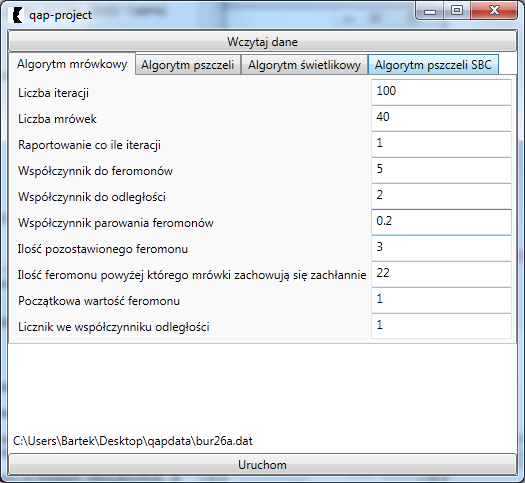
\includegraphics{aplikacja.png}
    }
W aplikacji na zakładce "Algorytm mrówkowy" znajdują się następujące możliwe do ustalenia parametry działania algorytmu:
\begin{itemize}
\item Liczba iteracji
\item Liczba mrówek
\item Raportowanie co ile iteracji -- co ile iteracji aktualny wynik ma się pojawiać na wykresie
\item Współczynnik do feromonów -- współczynnik wpływu feromonów na prawdopodobieństwo wyboru drogi - parametr $\alpha$ we wzorze \eqref{eqn:prawd_normal}
\item Współczynnik do odległości -- współczynnik wpływu odległości na prawdopodobieństwo wyboru drogi - parametr $\beta$ we wzorze \eqref{eqn:prawd_normal}
\item Współczynnik parowania feromonów -- współczynnik $\rho$ we wzorze \eqref{eqn:parowanie} z zakresu od 0 (brak parowania) do 1 (całkowite parowanie)
\item Ilość pozostawionego feromonu -- ilość feromonu, który zostawia po każdej iteracji mrówka, która znalazła najlepsze w danej iteracji rozwiązanie
\item Ilość feromonu powyżej którego mrówki zachowują się zachłannie -- ilość feromonu na ścieżkach, która powoduje, że mrówki wybierają kolejne węzły z prawdopodobieństwem \eqref{eqn:prawd_zachl}
\item Początkowa wartość feromonu -- wartość, jaką jest inicjalizowana macierz feromonów $\tau_{ij}$
\item Licznik we współczynniku odległości -- licznik Q we współczynniku $\eta$
\end{itemize}

\subsection{Testy algorytmu}
Poniżej przedstawiono kilka przykładowych wywołań algorytmu dla różnych~przykładowych~danych.

\begin{figure}
\resizebox{14cm}{!}{
      % wstawienie obrazka
      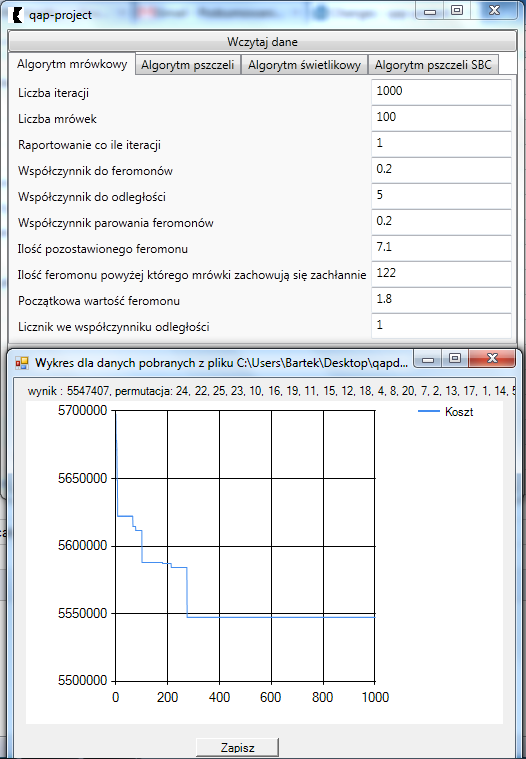
\includegraphics{wykres11.png}
}
\caption[Podpis_do_spisu]{Plik bur26a.dat - pierwszy zestaw parametrów (wynik optymalny: 5426670)}
\end{figure}

\begin{figure}
\resizebox{14cm}{!}{
      % wstawienie obrazka
      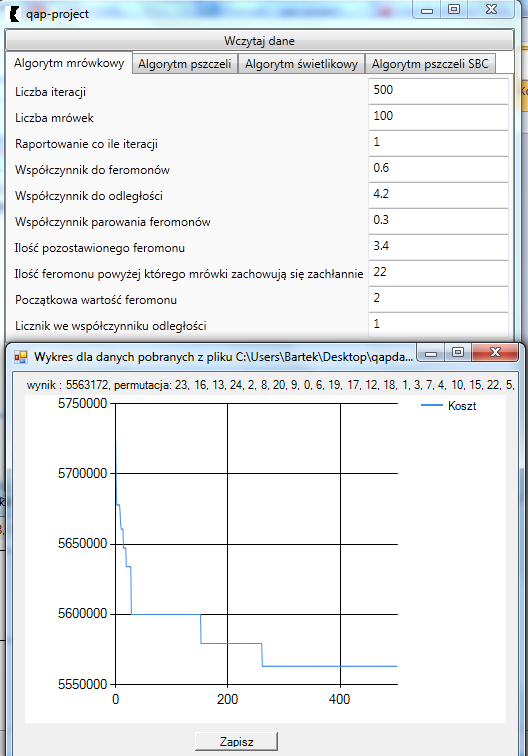
\includegraphics{wykres12.png}
}
\caption[Podpis_do_spisu]{Plik bur26a.dat - drugi zestaw parametrów (wynik optymalny: 5426670)}
\end{figure}

\begin{figure}
\resizebox{14cm}{!}{
      % wstawienie obrazka
      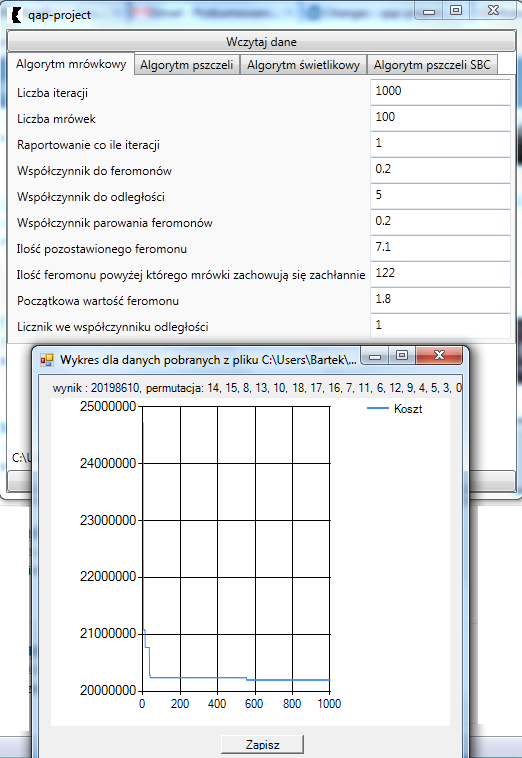
\includegraphics{wykres21.png}
}
\caption[Podpis_do_spisu]{Plik els19.dat - pierwszy zestaw parametrów (wynik optymalny: 17212548)}
\end{figure}

\begin{figure}
\resizebox{14cm}{!}{
      % wstawienie obrazka
      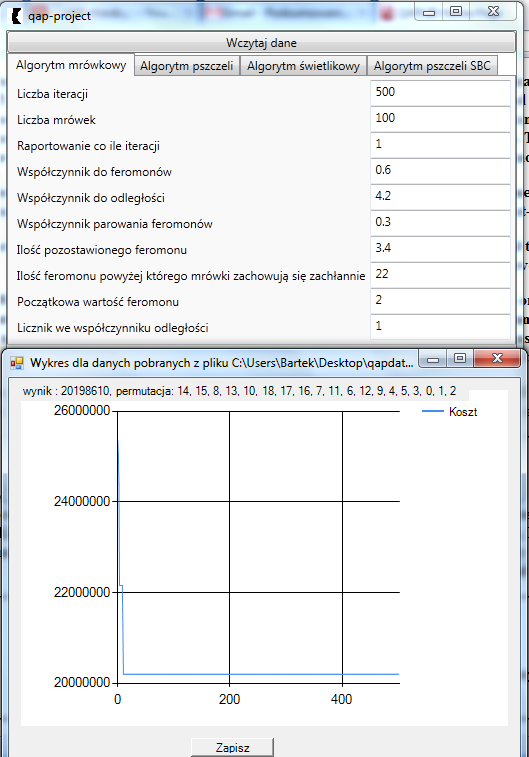
\includegraphics{wykres22.png}
}
\caption[Podpis_do_spisu]{Plik els19.dat - drugi zestaw parametrów (wynik optymalny: 17212548)}
\end{figure}

\begin{figure}
\resizebox{14cm}{!}{
      % wstawienie obrazka
      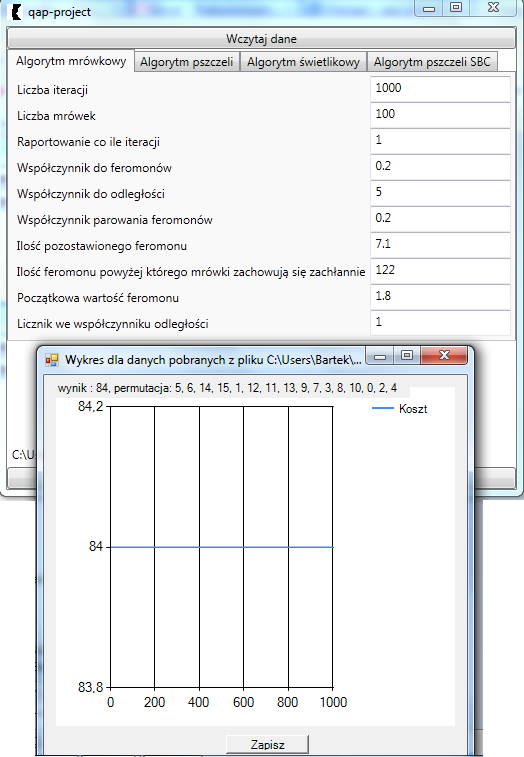
\includegraphics{wykres31.png}
}
\caption[Podpis_do_spisu]{Plik esc16a.dat - pierwszy zestaw parametrów (wynik optymalny: 68)}
\end{figure}

\begin{figure}
\resizebox{14cm}{!}{
      % wstawienie obrazka
      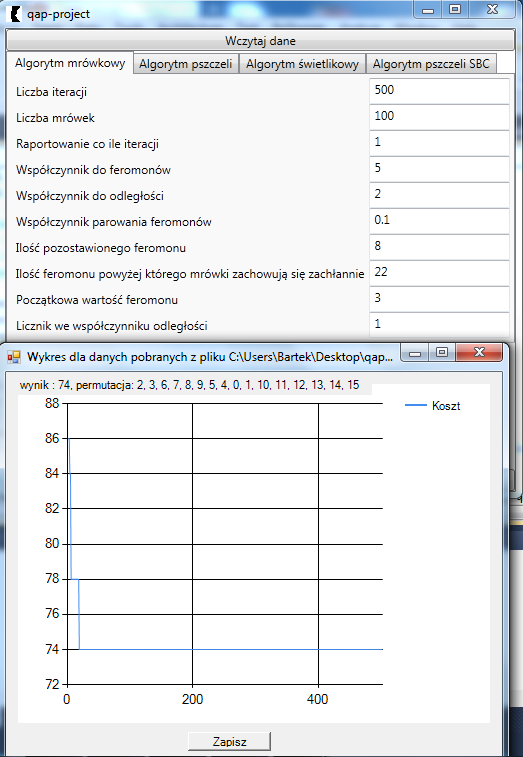
\includegraphics{wykres32.png}
}
\caption[Podpis_do_spisu]{Plik esc16a.dat - drugi zestaw parametrów (wynik optymalny: 68)}
\end{figure}

\end{document}
